% LTeX: language=de-CH

\section{Methodisches Vorgehen} \label{sec:methodik}

\subsection{Methodischer Ansatz der Studie}

\subsubsection{Echtzeiterhebungen mittels wiederholter Befragung (Experience Sampling)}

Die Erhebung von momentanen Wohlbefindenszuständen setzt methodisch voraus, dass subjektive Erfahrungen möglichst zeitnah und kontextsensitiv gemessen werden. Retrospektive Selbstberichte sind typischerweise anfällig für Verzerrungen, die durch selektive Erinnerung oder nachträgliche Neubewertungen entstehen (\textit{Recall Bias}), und daher nur begrenzt geeignet, um flüchtige affektive Zustände präzise abzubilden \parencite{kahnemanDevelopmentsMeasurementSubjective2006}. Als methodische Antwort auf diese Herausforderung etablierte sich das sogenannte Experience Sampling, auch als Ecological Momentary Assessment (\acrshort{ema}) bekannt. Dieser Ansatz basiert auf wiederholten, situativ eingebetteten Messungen, welche affektive, kognitive oder auch verhaltensbezogene Zustände unmittelbar während oder kurz nach dem Erleben erfassen \parencite{birenboimInfluenceUrbanEnvironments2018, kirchnerSpatiotemporalDeterminantsMental2016}.

In der vorliegenden Studie wird dieser methodische Zugang genutzt, um individuelle Wohlbefindenszustände und deren räumlichen Kontext systematisch zu erfassen. Durch den Einsatz einer eigens entwickelten Smartphone-Applikation erfolgt die Datenerhebung in Echtzeit und räumlich exakt, da neben der unmittelbaren affektiven Selbsteinschätzung auch Geolokationsdaten automatisiert gespeichert werden. Die Verwendung einer Smartphone-basierten Methodik erlaubt somit eine exakte Zuordnung von affektiven Zuständen zu spezifischen räumlichen Umgebungen. Damit folgt der methodische Ansatz aktuellen Empfehlungen der Forschung, wonach insbesondere die Kombination von Experience Sampling mit ortsbezogenen Daten (Geographically Explicit Ecological Momentary Assessment; \acrshort{gema}) eine differenzierte Analyse situativer und räumlicher Einflüsse auf das Wohlbefinden ermöglicht \parencite{mascherekMeadowsAsphaltRoad2025, kirchnerSpatiotemporalDeterminantsMental2016}.

Die Entscheidung für wiederholte Messungen innerhalb einer Person bietet gegenüber Querschnittstudien deutliche methodische Vorteile. Erstens erhöht die wiederholte intraindividuelle Datenerhebung die Präzision der Messungen und reduziert Verzerrungen, da interpersonelle Differenzen in der affektiven Bewertung von Situationen kontrolliert werden können. Zweitens erlaubt sie, kurzfristige Schwankungen und Dynamiken im Wohlbefinden abzubilden, die für langfristige Lebenszufriedenheitsskalen unerreichbar bleiben. Drittens bietet ein solches Studiendesign die Möglichkeit, situative Kontexteffekte unmittelbar zu analysieren und damit detailliert zu identifizieren, welche räumlichen Faktoren Wohlbefinden positiv oder negativ beeinflussen \parencite{birenboimInfluenceUrbanEnvironments2018, hammoudSmartphonebasedEcologicalMomentary2024}.

Zur Erfassung des momentanen Wohlbefindens wurden numerische Skalen eingesetzt, welche sowohl die Belastung der Teilnehmenden reduzieren als auch valide und vergleichbare Daten generieren \parencite{cookeMeasuringWellBeingReview2016}. Gleichzeitig erfolgte die automatische Erfassung räumlicher Kontexte mithilfe integrierter GPS-Funktionalitäten der eingesetzten mobilen Geräte. Dieses Design stellt sicher, dass subjektive Wahrnehmungen und objektive räumliche Kontextmerkmale präzise aufeinander bezogen analysiert werden können.

\subsubsection{Explorativer Charakter und Konsequenzen für die Auswertung}

Die vorliegende Studie verfolgt einen explorativen Forschungsansatz. Explorative Studien zeichnen sich dadurch aus, dass sie nicht primär auf Hypothesentests abzielen, sondern zunächst die systematische Erkundung neuer Zusammenhänge und methodischer Ansätze im Vordergrund steht. Insbesondere in Forschungsfeldern, in denen etablierte theoretische Modelle noch unzureichend vorhanden sind oder spezifische methodische Herausforderungen bestehen, ist ein exploratives Vorgehen angezeigt, um potenzielle theoretische oder empirische Lücken sichtbar zu machen und Hypothesen für zukünftige Forschung zu generieren \parencite{stebbinsExploratoryResearchSocial2001}.

Im Kontext dieser Studie begründet sich der explorative Ansatz einerseits aus der methodischen Innovation – der Verknüpfung von räumlichen und affektiven Echtzeit-Daten mittels einer neu entwickelten App – und andererseits aus der geringen Stichprobengrösse und der vergleichsweise niedrigen Rücklaufquote, welche umfangreiche inferenzstatistische Auswertungen begrenzen. Diese Limitationen erlauben keine generalisierenden Aussagen im Sinne klassischer Hypothesentestungen, sondern verlagern den Fokus auf die detaillierte Beschreibung und initiale Exploration möglicher Zusammenhänge zwischen räumlicher Umgebung, Wohlbefinden und intersektionaler Positionierung.

Konkret bedeutet dies für die Datenauswertung, dass der Schwerpunkt auf deskriptiven und explorativ-inferenzstatistischen Verfahren liegt. Analytisch kommen daher primär Verfahren wie explorative Visualisierungen, gemischte lineare Modelle (\acrshort{maihda}) und deskriptive Statistiken zum Einsatz. Gemischte lineare Modelle ermöglichen hierbei eine differenzierte Abbildung von Varianzanteilen auf individueller und gruppenspezifischer Ebene und erlauben somit, trotz geringer Stichprobengrössen, initiale Hinweise auf mögliche intersektionale Muster oder räumliche Unterschiede im Wohlbefinden aufzuzeigen \parencite{grossModellingIntersectionalityQuantitative2023, bauerIntersectionalityQuantitativeResearch2021}.

Zudem verlangt der explorative Charakter eine besonders kritische methodische Reflexion der Ergebnisse. Interpretation und Diskussion der Ergebnisse müssen explizit auf potenzielle methodische Grenzen hinweisen und die Befunde klar als vorläufig kennzeichnen. Der explorative Ansatz liefert somit vor allem wertvolle Ansatzpunkte und Hinweise für zukünftige Forschungsvorhaben, welche mithilfe grösserer Stichproben, verbesserter Rekrutierungsstrategien und methodischer Verfeinerungen auf den hier gewonnenen Erkenntnissen aufbauen könnten.


\subsection{Vergleich mit bestehenden Erhebungsinstrumenten}

\subsubsection{Tool A: Echtzeiterhebung ohne intersektionale Analyse}

Das \textit{Urban Mind}-Projekt\footnote{Siehe \url{https://www.urbanmind.info/}} stellt ein beispielhaftes Werkzeug dar, um subjektives momentanes Wohlbefinden in städtischen Kontexten mittels Echtzeiterhebungen systematisch zu erfassen und zu analysieren \parencite{bakolisUrbanMindUsing2018}. Es basiert auf einer mobilen Smartphone-App, die mithilfe von Ecological Momentary Assessment (EMA) detaillierte Einblicke in den Zusammenhang zwischen unmittelbaren Umweltfaktoren und mentalem Wohlbefinden ermöglicht.

Zentrales Anliegen des Urban Mind-Tools ist es, die Effekte spezifischer Naturelemente, wie beispielsweise Bäume, Himmel, Wasser oder Vogelgesang, auf das mentale Wohlbefinden in Echtzeit zu untersuchen. Hierfür werden Proband\:innen mehrmals täglich über einen Zeitraum von sieben Tagen aufgefordert, kurze standardisierte Fragen zu ihrer aktuellen Umgebung und ihrem momentanen Wohlbefinden zu beantworten \parencite{bakolisUrbanMindUsing2018}. Die Datenerhebung erfolgt sowohl mittels Selbsteinschätzungen der räumlichen und sozialen Umgebung als auch über Geodaten, welche automatisiert die exakte räumliche Verortung der Teilnehmer\:innen ermöglichen.

\begin{figure}[htbp]
    \centering
    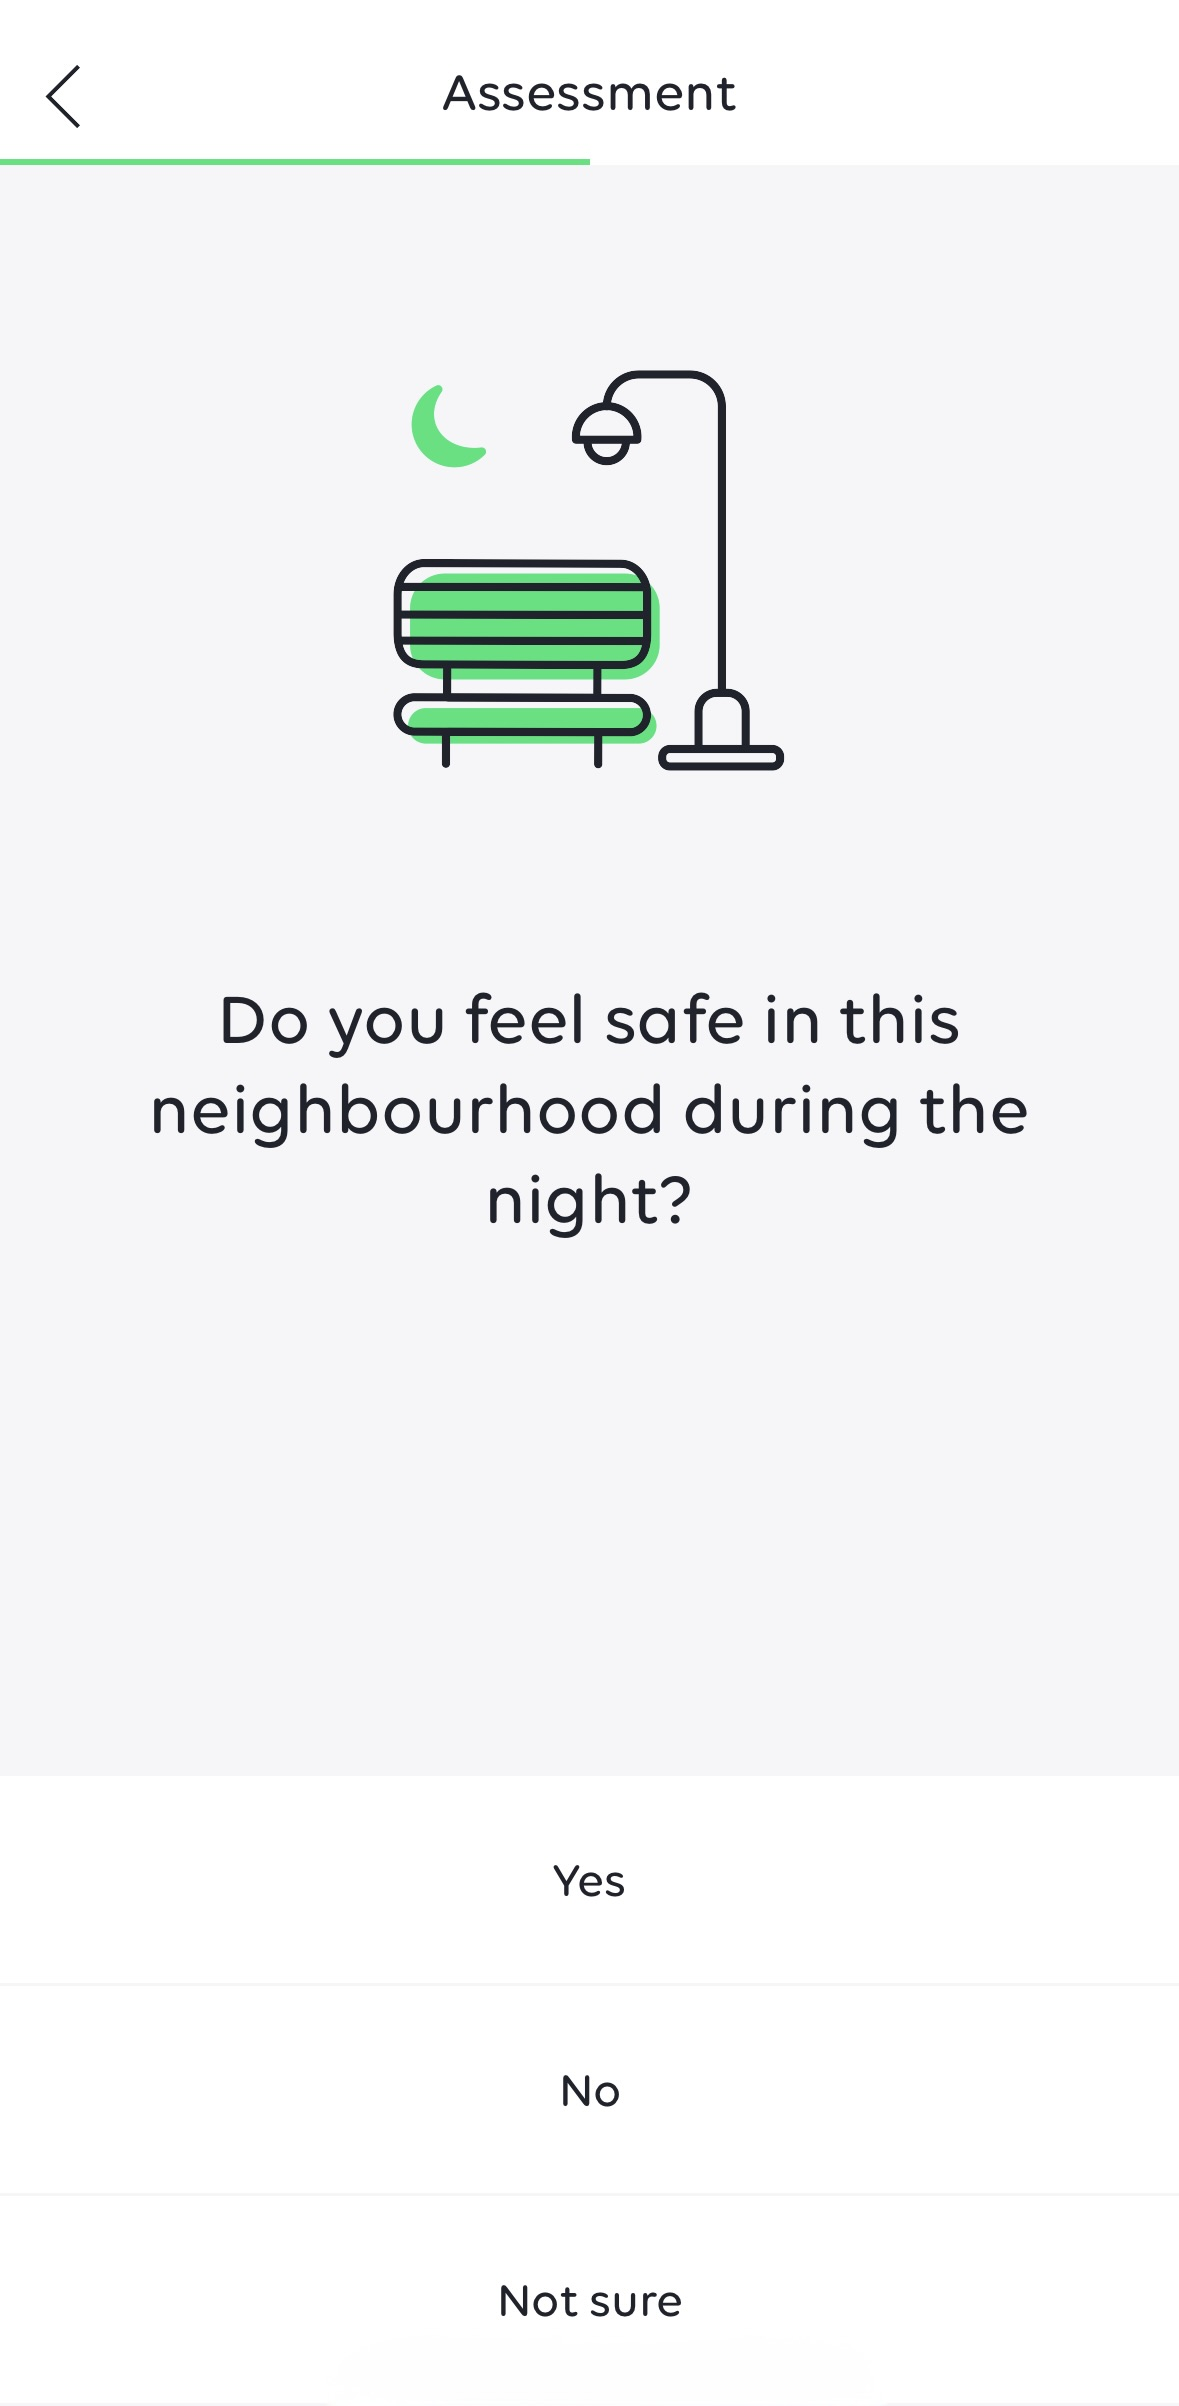
\includegraphics[width=0.5\textwidth]{Arbeit/images/urban_mind01.jpeg}
    \caption{Screenshot einer typischen Frageseite aus der Urban Mind-App}
    \label{fig:urban_mind_screenshot_1}
\end{figure}

Im Gegensatz zu traditionellen querschnittlichen Designs erlaubt das Urban Mind-Tool explizit die Analyse unmittelbarer und zeitverzögerter Effekte (Lag-Effekte). So konnten beispielsweise signifikant positive Effekte von Naturelementen wie Vogelgesang oder dem Sehen von Bäumen auf das momentane Wohlbefinden nachgewiesen werden, welche auch mehrere Stunden nach dem eigentlichen Naturkontakt noch messbar waren \parencite{bakolisUrbanMindUsing2018}. Darüber hinaus betont das Tool die Bedeutung individueller Differenzen und psychologischer Charakteristika, wie beispielsweise Impulsivität, die sich als moderierende Variable herausstellte: Personen mit höherer Impulsivität, welche typischerweise ein erhöhtes Risiko für psychische Erkrankungen aufweisen, profitieren stärker von unmittelbaren Naturerfahrungen.

Hinsichtlich des Designs und der Bedienbarkeit überzeugt die Urban Mind-App durch eine intuitive grafische Gestaltung sowie durch motivierende Elemente wie eine visuelle Übersicht über ausgefüllte und verpasste Fragebögen. Zudem ermöglicht sie Nutzer\:innen, ihre eigenen Daten retrospektiv aufzubereiten, was zu einer angeleiteten Reflexion des eigenen Wohlbefindens beiträgt. Dieses Feature unterstützt insbesondere eine nachhaltige und motivierte Teilnahme über den gesamten Erhebungszeitraum hinweg.

Obwohl Urban Mind zahlreiche methodische und technische Stärken aufweist, berücksichtigt es intersektionale Perspektiven bisher nicht explizit. So sind beispielsweise soziale Kategorien wie Geschlecht, Ethnizität oder sozioökonomischer Status zwar als demografische Variablen erfasst, werden jedoch nicht systematisch in einer intersektionalen Analyse miteinander in Beziehung gesetzt. Theoretisch wäre es möglich, intersektionale Analysen retrospektiv auf Grundlage der erhobenen Daten durchzuführen, eine solche methodische Perspektive wurde jedoch bislang nicht verfolgt.

Die im Rahmen dieser Bachelorarbeit entwickelte App teilt grundlegende methodische Prinzipien mit dem Urban Mind-Tool, wie insbesondere die Nutzung der \gls{ema}-Methode zur Echtzeiterhebung und die Integration räumlicher Kontextinformationen. Im Unterschied zu Urban Mind beinhaltet die entwickelte App jedoch zusätzliche methodische Elemente, wie etwa differenzierte Slider-Fragen, die eine feinere Abstufung subjektiver Empfindungen ermöglichen. Ferner sieht das methodische Konzept dieser Arbeit explizit eine intersektionale Auswertung vor, welche die Urban Mind-Studien in ihrer bisherigen Form nicht integriert haben.

Zusammenfassend lässt sich feststellen, dass Urban Mind in technischer und methodischer Hinsicht ein bewährtes und umfassend validiertes Tool darstellt, dessen methodische Grundprinzipien auch im Rahmen der hier vorliegenden Studie genutzt wurden. Gleichzeitig erweitert die vorliegende Arbeit diesen Ansatz um eine explizit intersektionale Perspektive, welche bisher im Kontext von Echtzeiterhebungen zu räumlichem Wohlbefinden noch unzureichend repräsentiert ist.

Zur Veranschaulichung und besseren Verständlichkeit der methodischen Unterschiede werden im Folgenden ausgewählte Screenshots der Urban Mind-App eingefügt (siehe \Cref{fig:urban_mind_screenshot_1} und Y). Diese zeigen exemplarisch die visuelle Gestaltung der Fragen sowie die ansprechende Übersicht der Teilnehmer\:innen über ihre beantworteten und verpassten Befragungseinheiten, welche als besonders motivierendes Element hervorzuheben sind \parencite{bakolisUrbanMindUsing2018}.

Dieser Vergleich verdeutlicht sowohl methodische Gemeinsamkeiten als auch Unterschiede zwischen den beiden Instrumenten und ermöglicht eine fundierte Einordnung der vorliegenden Studie innerhalb aktueller Ansätze zur Echtzeiterhebung von Wohlbefinden in urbanen Kontexten.


\subsubsection{Tool B: Retrospektive Erhebung und intersektionale Analyse mittels Relief Maps+}

Im Gegensatz zur App „Urban Mind“, die auf eine Echtzeit-Erfassung unmittelbarer Umgebungseinflüsse auf das mentale Wohlbefinden fokussiert, verfolgt das Tool „Relief Maps+“ von Rodó-de-Zárate und Kolleg\*innen einen retrospektiven, explizit intersektionalen Ansatz zur Analyse subjektiver Erfahrungen in unterschiedlichen Räumen und sozialen Kontexten. „Relief Maps+“ ist eine digitale Weiterentwicklung der ursprünglichen „Relief Maps“, die bereits 2014 von Rodó-de-Zárate als empirisches Werkzeug entwickelt wurden, um räumliche, soziale und emotionale Dimensionen intersektionaler Ungleichheiten qualitativ und quantitativ sichtbar zu machen\footnote{Siehe \url{https://reliefmaps.upf.edu/}} \parencite{rodo-de-zarateDevelopingGeographiesIntersectionality2014, luizdesouzaSpiralValidationProcess2025}.

Ziel der „Relief Maps+“ ist es, differenzierte Erfahrungen von Diskriminierung, Unterdrückung, aber auch Privilegien sichtbar zu machen, indem sie drei miteinander verwobene Dimensionen abbilden: die geografische Dimension (konkrete Orte oder räumliche Kontexte), die soziale Dimension (intersektionale Positionierungen wie Gender, Sexualität, Ethnizität oder Alter) und die emotionale Dimension (die subjektiven Gefühle der Teilnehmenden, z. B. Komfort oder Diskomfort). Dadurch werden Machtverhältnisse und deren Auswirkungen auf alltägliche Erfahrungen sowohl räumlich als auch sozial differenziert und emotional nachvollziehbar dargestellt \parencite{rodo-de-zarateIntersectionalitySpatialityEmotions2023}.

Im methodischen Vorgehen erfolgt die Datenerhebung retrospektiv durch ein Online-Formular, in dem die Teilnehmenden ihre subjektiven Erfahrungen in unterschiedlichen sozialen Situationen und an verschiedenen Orten beschreiben. Dabei bewerten sie explizit ihr emotionales Erleben, beispielsweise anhand einer Skala von Komfort zu Diskomfort, und ordnen diese Erfahrungen verschiedenen intersektionalen Positionen (z. B. Geschlecht, Sexualität oder Ethnizität) zu. Daraus resultieren sogenannte „Relief Maps“, die visuell darstellen, an welchen Orten und unter welchen sozialen Bedingungen Diskriminierung oder Privilegierung erlebt wurde \parencite{luizdesouzaSpiralValidationProcess2025, rodo-de-zarateIntersectionalitySpatialityEmotions2023}.

Ein wichtiger Vorteil dieses Ansatzes ist die bewusste und explizite Integration von Reflexivität und Positionalität, da Teilnehmende aufgefordert werden, ihre Erfahrungen in Bezug zu ihren eigenen sozialen Positionierungen kritisch zu reflektieren. „Relief Maps+“ wurde überdies durch ein umfassendes Validierungsverfahren entwickelt, das qualitative, feministische und intersektionale Perspektiven konsequent integrierte. Dabei spielten iterative Feedbackprozesse, Diskussionsgruppen und Pilotstudien eine entscheidende Rolle, um eine ethisch fundierte und theoretisch konsistente Methodik zu gewährleisten \parencite{luizdesouzaSpiralValidationProcess2025}.

Zentraler Aspekt der theoretischen Fundierung von „Relief Maps+“ ist zudem die differenzierte Betrachtung von Emotionen im Zusammenhang mit intersektionalen Ungleichheiten. Gemäss Rodó-de-Zárate fungieren Emotionen als Indikatoren für soziale Positionierungen und Machtverhältnisse, wobei zwischen systematischen Diskomforts, situativen Diskomforts sowie ethischen Diskomforts unterschieden wird. Diese emotionale Perspektive erlaubt es, die komplexen Wechselwirkungen von Orten, sozialen Identitäten und emotionalen Erfahrungen methodisch erfassbar und theoretisch interpretierbar zu machen \parencite{rodo-de-zarateIntersectionalitySpatialityEmotions2023}.

In der Visualisierung der Ergebnisse ermöglichen „Relief Maps+“ die Darstellung von Erfahrungen sowohl individueller als auch gruppenbezogener Art. Die Karten veranschaulichen, wie bestimmte soziale Positionierungen, etwa Geschlecht oder Sexualität, in spezifischen Kontexten systematisch mit Diskriminierung oder Privilegien verbunden sind. Besonders hervorzuheben ist dabei die Fähigkeit des Tools, simultan mehrere Achsen der Unterdrückung und deren räumlich-emotionale Variabilität sichtbar zu machen \parencite{rodo-de-zarateDevelopingGeographiesIntersectionality2014}.

Verglichen mit dem Tool „Urban Mind“ stellt „Relief Maps+“ somit eine tiefer gehende und differenziertere Methodik dar, um intersektionale Dynamiken retrospektiv sichtbar zu machen. Während „Urban Mind“ primär auf unmittelbare Umwelteinflüsse fokussiert und dabei soziale Positionierungen weitgehend unberücksichtigt lässt, setzt „Relief Maps+“ explizit auf eine komplexe intersektionale Perspektive, um systemische und strukturelle Ungleichheiten sichtbar zu machen. Der retrospektive Ansatz erlaubt dabei eine gründliche Reflexion der eigenen Erfahrungen und der sie prägenden gesellschaftlichen Strukturen, bietet allerdings nicht die hohe ökologische Validität und unmittelbare Reaktivität von Echtzeit-Ansätzen wie bei „Urban Mind“.

Für die vorliegende Studie bedeutet dies, dass beide Tools wichtige Anregungen bieten, jedoch unterschiedliche Stärken aufweisen: „Urban Mind“ durch den unmittelbaren, ökologisch validen Zugang zu Alltagserfahrungen, „Relief Maps+“ durch die explizite Integration komplexer intersektionaler Zusammenhänge und deren theoretisch fundierte, räumlich-emotionale Analyse. Beide Perspektiven ergänzen sich methodisch und analytisch, wodurch ein tiefergehendes Verständnis des räumlich situierten, intersektionalen Wohlbefindens erreicht werden kann.


\subsubsection{Einordnung des eigenen Ansatzes}

Die vorliegend entwickelte App greift das Grundprinzip von \emph{Urban Mind} – die mehrfach tägliche Erhebung subjektiver Befindlichkeiten \emph{in situ} – auf und erweitert es in zwei zentralen Punkten:

\begin{enumerate}
    \item \textbf{Methodische Flexibilität.} Neben Single- und Multiple-Choice-Items stehen kontinuierliche Schieberegler sowie optionale Freitextfelder zur Verfügung. Dadurch lassen sich sowohl feingranulare quantitative Einschätzungen als auch kontextspezifische qualitative Informationen erfassen. Die zugrunde liegende React-Native-Codebasis ist modular aufgebaut; neue Fragetypen können mit minimalem Programmieraufwand ergänzt werden.

    \item \textbf{Explizit intersektionale Ausrichtung.} Während \emph{Urban Mind} soziale Kategorien lediglich in der Baseline erfasst, verknüpft der hier gewählte Ansatz zwei Ebenen systematisch: \textit{(i)} detaillierte, einmalig erhobene Soziodemografie (Alter, zugewiesenes und selbstidentifiziertes Geschlecht, sexuelle Orientierung, Behinderung, Einkommen u.\,a.) und \textit{(ii)} situative EMA-Items, die gezielt nach etwaigen Einflüssen eben dieser Merkmale auf das aktuelle Wohlbefinden fragen. Damit wird Intersektionalität nicht nur retrospektiv–korrelativ, sondern \emph{situativ-explizit} operationalisiert.
\end{enumerate}

Die Kombination beider Ebenen erlaubt eine mehrdimensionale Modellierung: Baseline-Merkmale definieren strukturelle Ausgangspositionen, situative Angaben erfassen konkrete Erfahrungen. Durch lineare Mixed-Models oder MAIHDA-Ansätze lassen sich Wechselwirkungen zwischen sozialen Positionen, räumlichen Kontexten und momentanen Befindlichkeiten quantitativ abbilden; Freitextangaben liefern zugleich reichhaltiges Material für eine kontextualisierende, qualitative Vertiefung.

\subsection{Beschreibung der entwickelten App}

\subsubsection{Konzept und Funktionalität}

\textit{InterMind} wurde als leichtgewichtige, datensparsame Research-App konzipiert, deren Architektur funktionale und nicht-funktionale Anforderungen klar trennt.

\paragraph{Funktionale Anforderungen}

\begin{itemize}
  \item \textbf{Pseudonyme Geräte-ID} anstelle persönlicher Konten (privacy by design).
  \item \textbf{Experience-Sampling (EMA):} drei randomisierte Push-Prompts pro Tag.
  \item \textbf{Automatische Georeferenzierung} bei jeder Befragung.
  \item \textbf{Flexibles Fragebogensystem} mit Single-/Multiple-Choice, Slidern und Freitext.
  \item \textbf{Nutzerseitige Datenkontrolle} – lokales Löschen sämtlicher App-Daten jederzeit möglich.
\end{itemize}

\paragraph{Nicht-funktionale Anforderungen}

\begin{itemize}
  \item \textbf{Datenschutz \& Sicherheit:} Ende-zu-Ende-Verschlüsselung, DSG- DSGVO-konforme Pseudonymisierung.
  \item \textbf{Mehrsprachigkeit} (derzeit Deutsch / Englisch, erweiterbar).
  \item \textbf{Plattformkompatibilität} – Entwicklung mit \texttt{React Native + Expo}; Backend auf \texttt{Supabase} für skalierbare Postgres-Datenhaltung.
\end{itemize}

\subsubsection{Technische Umsetzung}

Beim ersten Start generiert die App eine randomisierte UUID, die lokal persistent gespeichert wird. Push-Benachrichtigungen werden clientseitig geplant und serverseitig via Supabase Functions verwaltet. Der Fragebogen wird aus einer JSON-Konfigurationsdatei geladen; neue Items können Forschende somit ohne Codeänderung ergänzen. Alle Nutzerdaten werden unmittelbar nach Upload aus dem Mobilgerät entfernt, sodass bei Verlust des Endgeräts keine sensitiven Informationen vorliegen.

Die schlanke UI (Abb.~\ref{fig:homescreen}) beschränkt sich auf drei Hauptansichten: \textit{Home} (Teilnahmestatus), \textit{Fragebogen} und \textit{Datenschutz}. Die Slider-Skalen sind bewusst farbneutral gehalten, um semantische Wertungen zu vermeiden; beim Freitextfeld ermöglicht ein Soft-Limit von 200 Zeichen knappe, kontextspezifische Kommentare.

Die so realisierte Architektur gewährleistet eine robuste, zugleich erweiterbare Grundlage für die geplante Mixed-Methods-Auswertung intersektionalen Wohlbefindens im Stadtraum.


\subsubsection{Fragebogenstruktur und Operationalisierung}

Der Fragebogen besteht aus zwei zentralen Elementen:

\paragraph{Baseline-Befragung (einmalig):}
Hier wurden grundlegende demografische Variablen (Alter, Geschlecht, sexuelle Orientierung, Behinderung, sozioökonomischer Hintergrund) erhoben, um soziale Positionierungen für spätere intersektionale Analysen verfügbar zu machen. Fragen wurden bewusst offen oder mit freier Spezifikation gestaltet, um Normativität in den Antwortoptionen zu vermeiden und soziale Positionierungen differenziert erfassen zu können.

\paragraph{Situative Befragung (wiederholt):}
Der wiederholt eingesetzte Fragebogen besteht aus kurzen situativen Erhebungen, die mittels EMA durchgeführt wurden. Teilnehmer:innen wurden regelmässig aufgefordert, Fragen zu ihrem momentanen Wohlbefinden (z.\,B. empfundene Sicherheit, Zugehörigkeit, Entspannung) sowie zur aktuellen räumlichen und sozialen Umgebung zu beantworten. Hierbei kamen insbesondere Slider-Fragen zum Einsatz, um eine kontinuierliche Bewertung zu ermöglichen. Ergänzend wurde ein optionales Freitextfeld angeboten, das qualitative Kontextinformationen und subjektive Reflexionen zuliess.

Der Begriff \emph{Operationalisierung} bezeichnet hierbei die konkrete Umsetzung theoretischer Konstrukte in messbare Indikatoren. Wohlbefinden wurde operationalisiert über sieben zentrale Dimensionen (u.\,a. Entspannung, Sicherheit, Zugehörigkeit), die in der Literatur als relevant identifiziert wurden. Räumliche und soziale Kontexte wurden mit Items operationalisiert, die beispielsweise aus der Forschung von Bakolis et al. (2018) übernommen und für die vorliegende Studie adaptiert wurden.

\subsubsection{Ablauf und Durchführung der Datenerhebung}

Die Datenerhebung fand im Rahmen der einführenden Exkursion „Recht auf Stadt“ im ersten Studienjahr des Bachelorstudiengangs Geographie an der Universität Bern im Mai 2025 statt. Die teilnehmenden Studierenden wurden zu Beginn der Exkursion über Zielsetzung und Ablauf informiert und konnten anschliessend freiwillig an der Befragung teilnehmen. Die Nutzung der App wurde über den gesamten Exkursionszeitraum von drei Tagen durchgeführt, wobei die Teilnehmenden via Push-Benachrichtigungen mehrfach täglich aufgefordert wurden, die kurzen situativen Befragungen auszufüllen. Die Baseline-Befragung erfolgte einmalig zu Beginn.

Die Durchführung im Exkursionssetting ermöglichte eine kontrollierte Testung der technischen Funktionalität und eine hohe Compliance bei den Teilnehmenden. Gleichzeitig erlaubte dieses Setting, reale räumliche Kontexte, wie unterschiedliche urbane Umgebungen in Zürich, Basel und Bern, unmittelbar in die Datenerhebung einzubeziehen. Insgesamt zeichneten sich die Daten durch eine hohe räumliche und kontextuelle Varianz aus, die zentrale Grundlage für die späteren intersektionalen Analysen bildete.

Die vollständigen Fragebögen (Baseline- und situative Befragungen) sind als ergänzende Dokumentation digital im GitHub-Repository der App hinterlegt. Dies folgt dem Prinzip offener und transparenter Forschung. Eine detaillierte Fragebogenübersicht kann zusätzlich im Anhang dieser Arbeit eingesehen werden, um die inhaltliche Struktur und die Operationalisierung der theoretischen Konstrukte nachvollziehbar zu machen.

Zusammenfassend stellt die entwickelte App somit ein methodisch differenziertes, technisch flexibles Instrument dar, das sowohl situative Dynamiken als auch intersektionale soziale Strukturen systematisch erfassbar macht. Die enge Verknüpfung mit einem explizit intersektional ausgerichteten Fragebogen ermöglicht es, bestehende methodische Ansätze (Urban Mind, Relief Maps+) gezielt zu erweitern und dabei neue Erkenntnisse zur Beziehung von Raum, Wohlbefinden und sozialer Positionierung zu generieren.


\subsection{Limitationen und Herausforderungen der Datenerhebung}

\subsubsection{Geringe Rücklaufquote und mögliche Ursachen}

\subsubsection{Auswirkungen auf die Datenqualität und Analyse}
